\subsection{The rebalance and smear method}

\section{Background information}
Purely hadronic events originating from QCD interactions in proton-proton collisions account for the vast majority of events observed at the LHC. Not surprisingly, these events are a major background to new physics signals that may manifest in the hadronic channel. Several features of QCD events are poorly modeled in simulation \ref{bib:thaler}, including the production cross section, jet multiplicity, and relationships between the directions of jets. This motivates the development of data-driven approaches to QCD estimation. Typically, approaches take advantage of the particularly well-modeled aspects of simulation, but rely on the data to model as many features as possible. As with any data-driven approach the method must be robust against possible signal contamination that may enter into control regions. 

Many data-driven approaches to QCD estimation take advantage of the fact that the only stable particles in the $\SM$ that are invisible to the CMS detector are neutrinos. Apart from rare final states containing heavy-flavor jets,  QCD events are free of neutrinos, and therefore exhibit little or no \MET at the parton level.  For this reason, the \MET typically serves as an excellent discriminating variable between the large QCD background and new physics models with significant \MET, such as models of R-parity conserving supersymmetry. However, QCD {\it only} exhibits zero \MET at the parton level $(\met)_{\rm part}$. The final-state particles are detected by a tracker and calorimeters with finite momentum and energy resolution, which means that estimates of each parton's momentum are only approximate. Small mis-measurements of the jet momenta propagate into the measured missing transverse energy, inducing a sometimes significant missing transverse energy measurement $(\met)_{\rm meas}$.  These statements are be expressed in the form of the following equations:
\begin{align}
%\begin{split}
(\vec{E}_{ T}^{\rm miss})_{\rm part} &\equiv -\sum_{i=1}^{n}(\vec{p}_{T})_{i,\rm parton\ }=0\\
(\vec{E}_{ T}^{\rm miss})_{\rm meas} &\equiv -\sum_{i=1}^{n}(\vec{p}_{T})_{i,\rm meas\ \ \ }\neq 0,
%\end{split}
\label{eq:metTrue}
\end{align}
where $i$ is the particle index and $n$ is the number of particles in the event.

\subsection{Model assumptions and likelihood} 
Assuming that jets differ between the parton and reconstruction levels in the magnitudes of their four-vectors, but not in their directions, the following expression relates the two stages of the jet collection of a given event:
\begin{equation}
\vec{J}_{\rm meas} = \hat{C} \vec{J}_{\rm part},
\end{equation}
where $\vec{J}_{\rm meas}$ and $\vec{J}_{\rm part}$ are $n\times 1$ vectors of the reconstructed jet four-vectors and the parton-level jet four-vectors, and $\hat{C}$ is diagonal $n\times n$ matrix whose elements are the jet energy scale factors $(c_1,c_2,...,c_n)$. The likelihood for a scale factor $c_i$, given by
\begin{equation}
L_{i}\equiv{\rm P}(c_i\ |\ p^{\mu}_{i,\rm part})={\rm P}(p^{\mu}_{i,\rm meas}|\ c_{i}),
\label{eq:JetEnergyLikelihood}
\end{equation}
is derived from simulation as the distribution of the ratio of parton-level jet momentum to the associated reconstruction-level jet momentum. The association of parton- and reconstruction-level jets is accomplished through the matching criterion,
\begin{equation}
\Delta R(p^{\mu}_{\textrm meas},p^{\mu}_{\textrm parton})<0.4.
\end{equation}	
Additionally, an isolation criterion,
\begin{equation}
p_{\rm T}/\sum_{i=1}^{\njets}[(p_{\rm T})_{i}\cdot\Theta(0.5-\Delta R(p^{\mu}_{i},p^{\mu}))]<1.01,
\end{equation}
is applied both to the parton-level jet collection and to the reconstruction-level jets in the selection of jets contributing to the likelihood. The likelihood, as shown in Figure \ref{fig:SmearEx}, is derived in bins of parton-level jet $p_T$ and $\eta$.
\begin{figure}[h]
\centering
\subfloat[]{
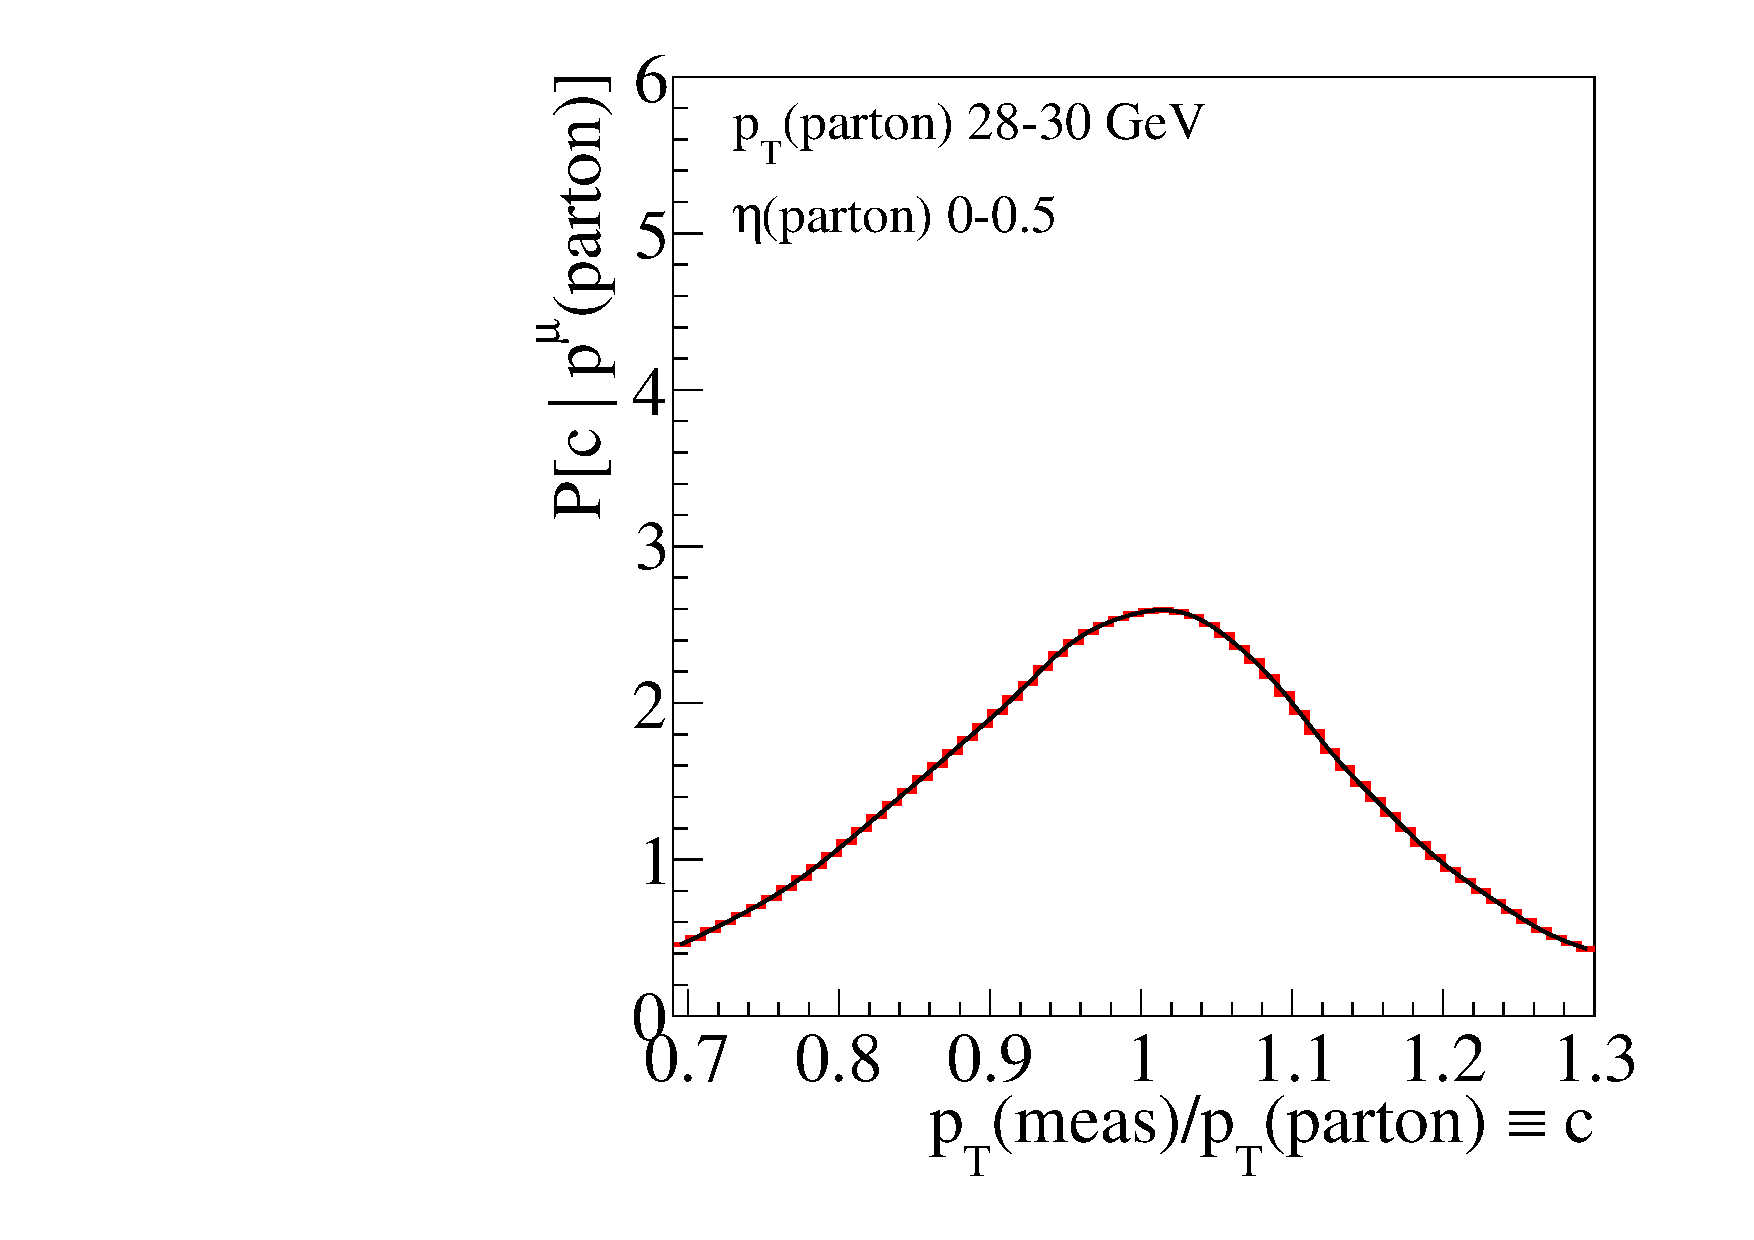
\includegraphics[width=0.5\linewidth]{figures/SusySearches/Ra2b2016/SmearEx1.pdf}
}
\subfloat[]{
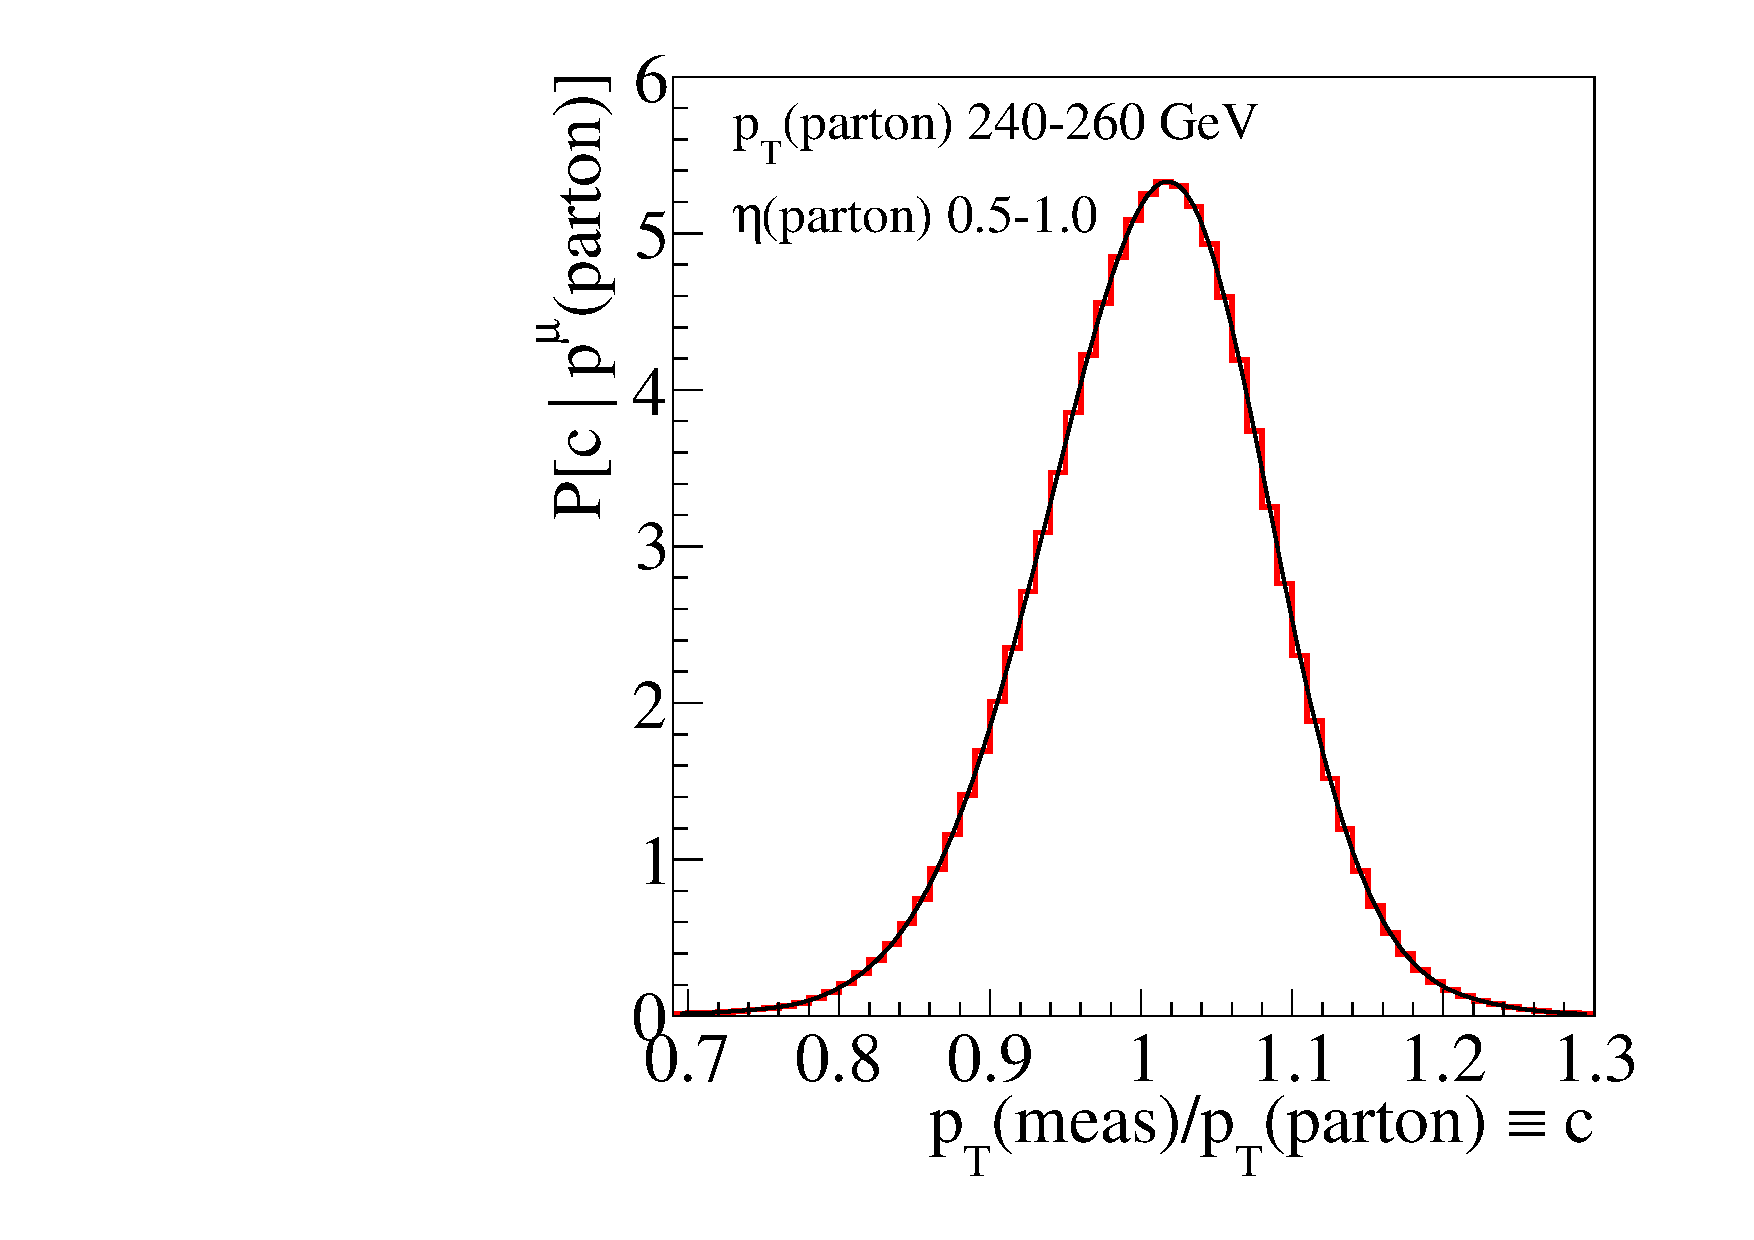
\includegraphics[width=0.5\linewidth]{figures/SusySearches/Ra2b2016/SmearEx2.pdf}
}
\caption{The likelihood function for the jet energy scale factor in two regions of the phase space of the parton-level jet four-vector. These distributions are equivalent to the smearing templates. The histograms (red) are smoothly interpolated using splines (black).}
\label{fig:SmearEx}
\end{figure}


\subsection{Rebalance and smear method}
The rebalance and smear method exploits the relationships given in Equations \ref{eq:metTrue}, along with jet energy scale (JES) factors, to form a transfer function between the measured and parton-level jets. The first stage of the method is to identify the optimal matrix of scale factors $\hat{C}$ that transforms the collection of reconstruction-level jets into a set that resembles a parton-level jet collection; jets in the resulting collection are referred to as the rebalanced jets. In the second stage, the four-vectors of the rebalanced jets are smeared according to the the likelihood for the JES factor given in Equation \ref{eq:JetEnergyLikelihood}. This procedure, applied to all events in a QCD-enriched data control sample, yields the prediction event sample. Predictions for the QCD background counts in the analysis signal regions are derived from placing cuts on the prediction event sample. Now for a closer look at each step.

\subsection{Rebalance procedure}
The objective is to rebalance the collection of measured jets so that it resembles a parton-level collection. An inversion of the likelihood function for the jet energy scale factors is performed using Bayes' theorem. The probability density for the parton-level jet collection can be written as
\begin{equation}
{\rm P}(\vec{J}_{\rm part}|\vec{J}_{\rm meas}) \sim {\rm P}(\vec{J}_{\rm meas}|\vec{J}_{\rm part})\cdot \pi(\vec{J}_{\rm part}),
\label{eq:posterior1}
\end{equation}
where $\pi(\{p^{\mu}_{i,\rm parton}\})$ is the $n$-dimensional prior probability density for the parton-level jet collection.
Treating the jets as independent from each other allows the likelihood to be factorized as
\begin{align}
\begin{split}
{\rm P}(\vec{J}_{\rm meas}|\vec{J}_{\rm part}) = \prod_{i=1}^{\njets}L_{i} &= \prod_{i=1}^{\njets}{\rm P}(p^{\mu}_{i,\rm meas}\ |\ p^{\mu}_{i,\rm part})\\
&= \prod_{i=1}^{\njets}{\rm P}(c_i\ |\ p^{\mu}_{i,\rm part})=\prod_{i=1}^{\njets}{\rm P}(p^{\mu}_{i,\rm meas}|\ c_{i}).
\end{split}
\label{eq:likelihood1}
\end{align}
The prior allows the probability density to be constrained by our knowledge about the parton-level missing transverse energy outlined in Equation \ref{eq:metTrue}. However, while equations \ref{eq:metTrue} are true for the $E_{T}^{\rm miss}$, the analysis at hand uses the missing transverse hadronic energy $\mht$, defined as
\begin{equation}
\vec{H}_{T}^{\rm miss} \equiv -\sum_{i=1}^{{\rm N}_{\rm jet}}(\vec{p}_{T})_{i}\cdot\Theta(30{\rm\ GeV}-(p_{T})_{i}).
\end{equation}
The threshold on the $p_{T}$ applied via the Heaviside theta serves to remove jets originating from pileup interactions, but also renders the equality in equation \ref{eq:metTrue} only approximate. Jets with $p_{T}$ less than 30 GeV can recoil off of harder jets, and this produces non-zero true $\mht$. However, the parton-level $\mht$ is still small compared to the reconstruction-level $\mht$, as seen in the distribution of parton- and reconstruction-level $\mht$ in Figure \ref{fig:Mht}. Also shown is the angular distribution of the $\mht$.
\begin{figure}[h]
\centering
\subfloat[]{
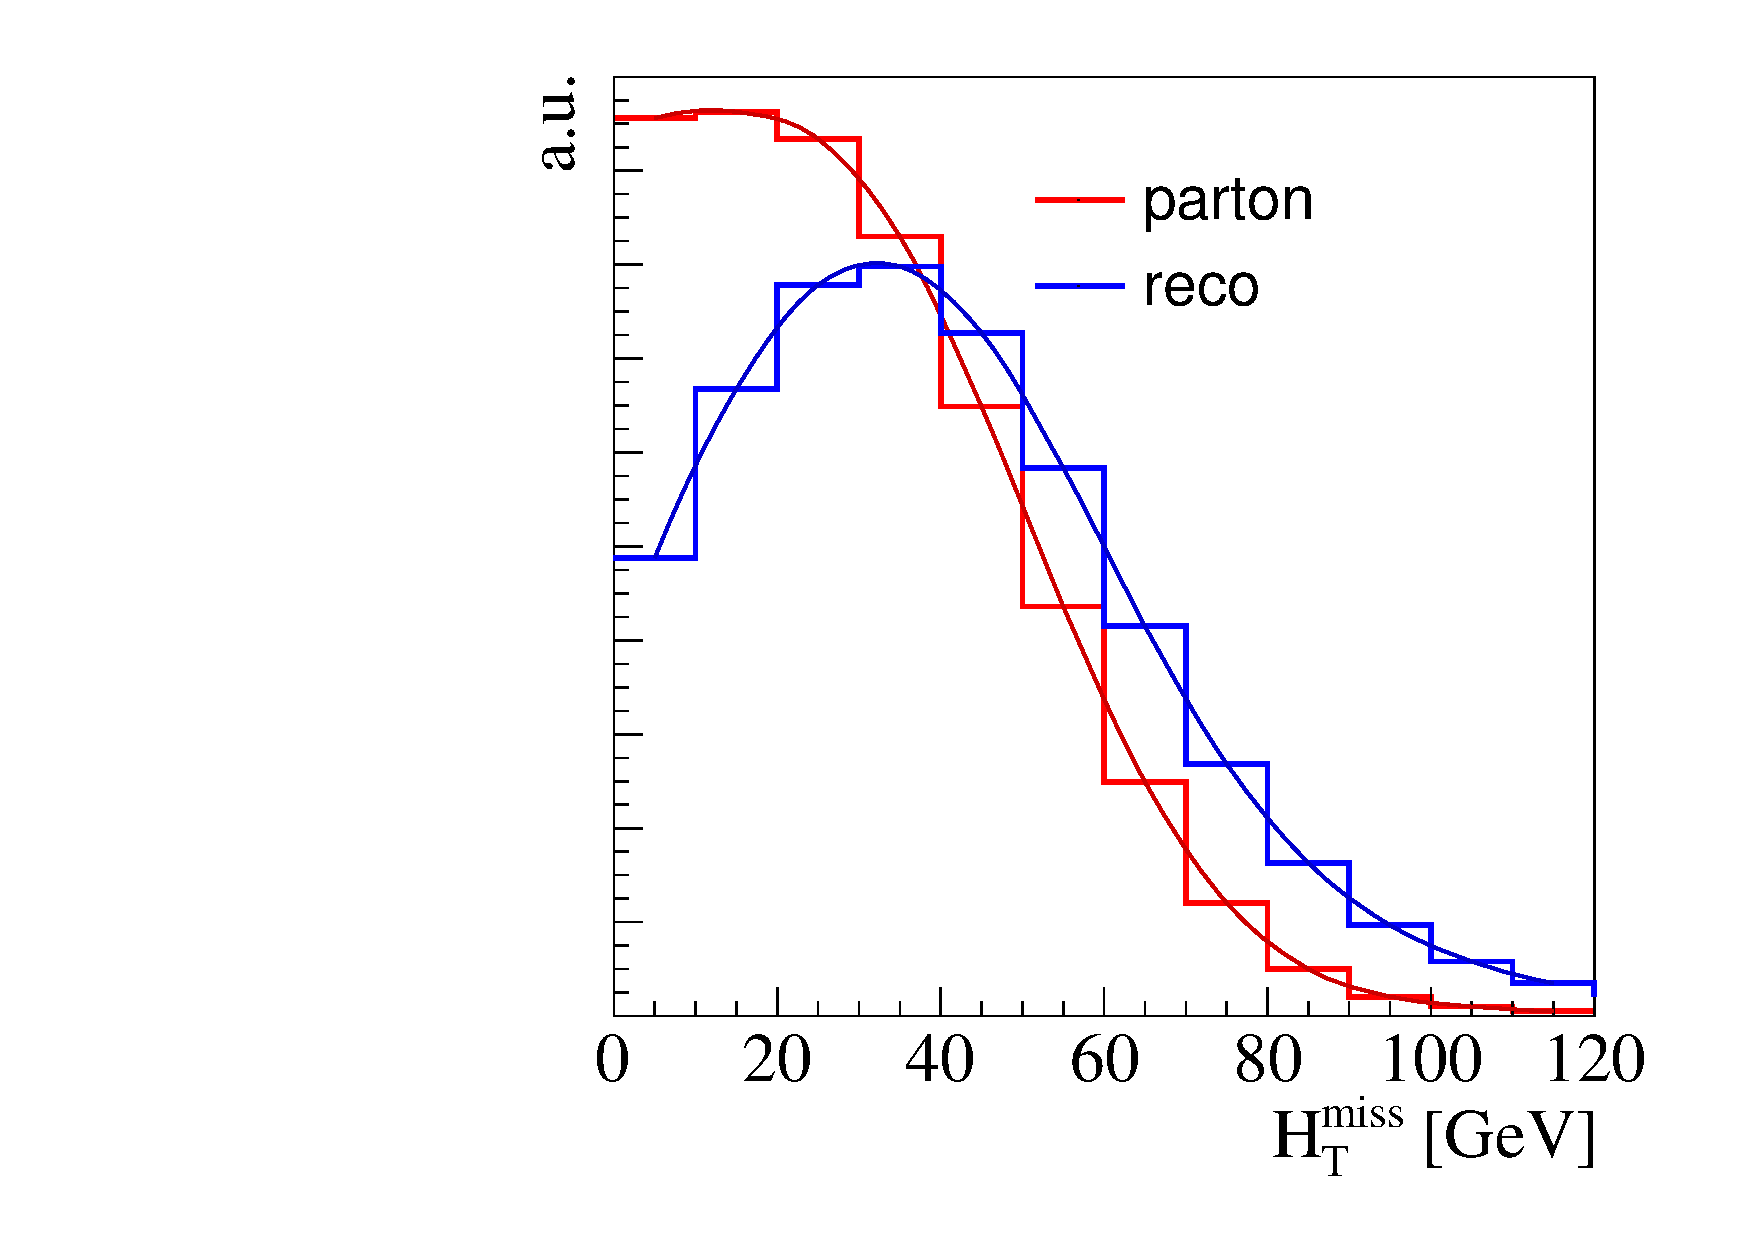
\includegraphics[width=0.5\linewidth]{figures/SusySearches/Ra2b2016/MhtGenAndTruth.pdf}
}
\subfloat[]{
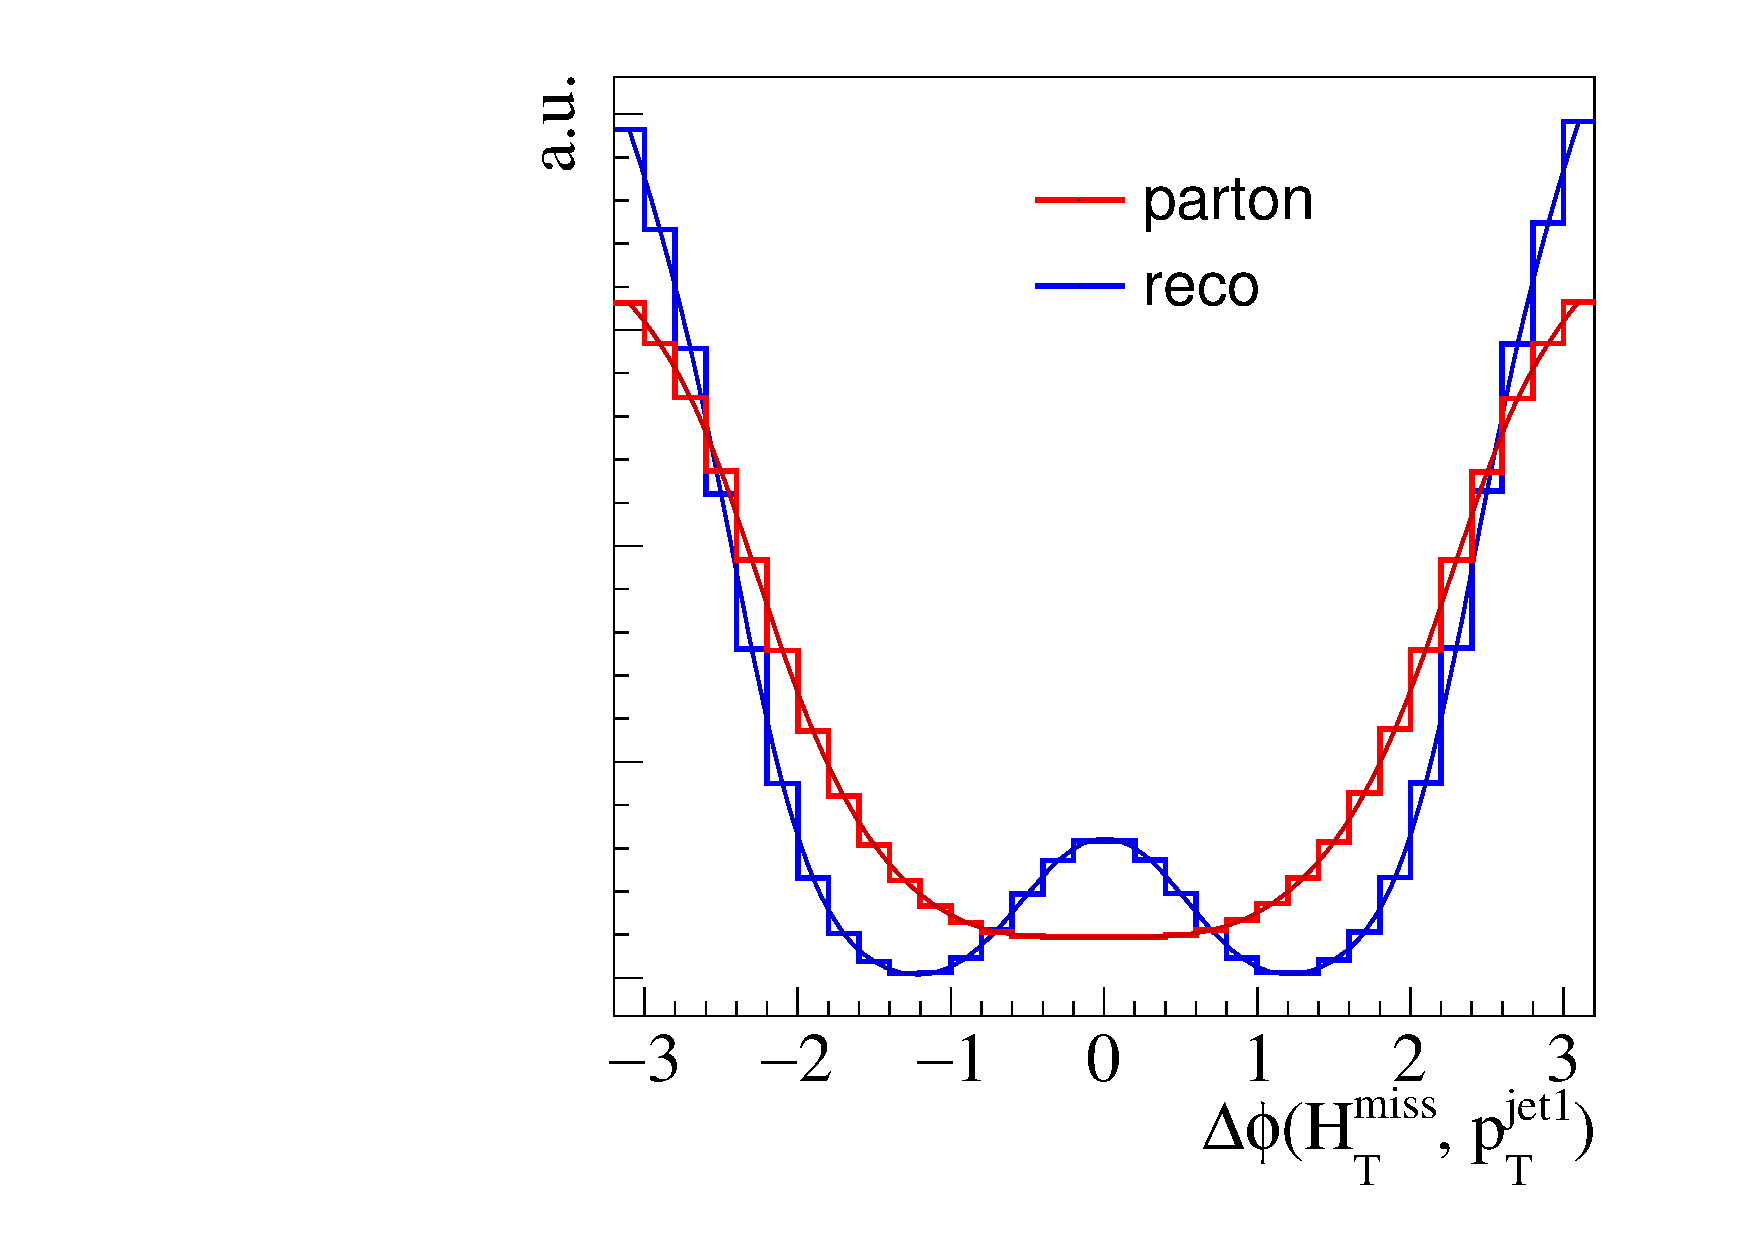
\includegraphics[width=0.5\linewidth]{figures/SusySearches/Ra2b2016/DPhiMhtJet1GenAndTruth.pdf}
}
\caption{The parton-level and reconstruction-level $\mht$ and azimuthal separation between the $\mht$ and leading jet in QCD simulation.}
\label{fig:Mht}
\end{figure}
the parton-level information contained in the red distributions can be incorporated into the posterior density via an expression relating the $\mht$ to the jet energy scale factors, and taking the red distributions to be factors in the prior. Combining Eqs. \ref{eq:posterior1}, \ref{eq:likelihood1} gives
\begin{equation}
{\rm P}(\vec{J}_{\rm part}|\vec{J}_{\rm meas}) \sim
\prod_{i=1}^{\njets}{\rm P}(p^{\mu}_{i,\rm meas}|\ c_{i})\cdot \mht(\vec{J}_{\rm part})\cdot \Delta\phi_{\mht,p_{T}^1}(\vec{J}_{\rm part})\cdot \pi_0(\vec{J}_{\rm part}),
\end{equation}
where $\pi_0(\vec{J}_{\rm part})$ is the initial prior on the parton jet four-vectors, taken to be uniform.


\subsection{Closure}

\begin{figure}[h]
\centering
\subfloat[]{
\includegraphics[width=0.5\linewidth]{figures/SusySearches/Ra2b2016/RplusSAndTruth_Ht.pdf}
}
\subfloat[]{
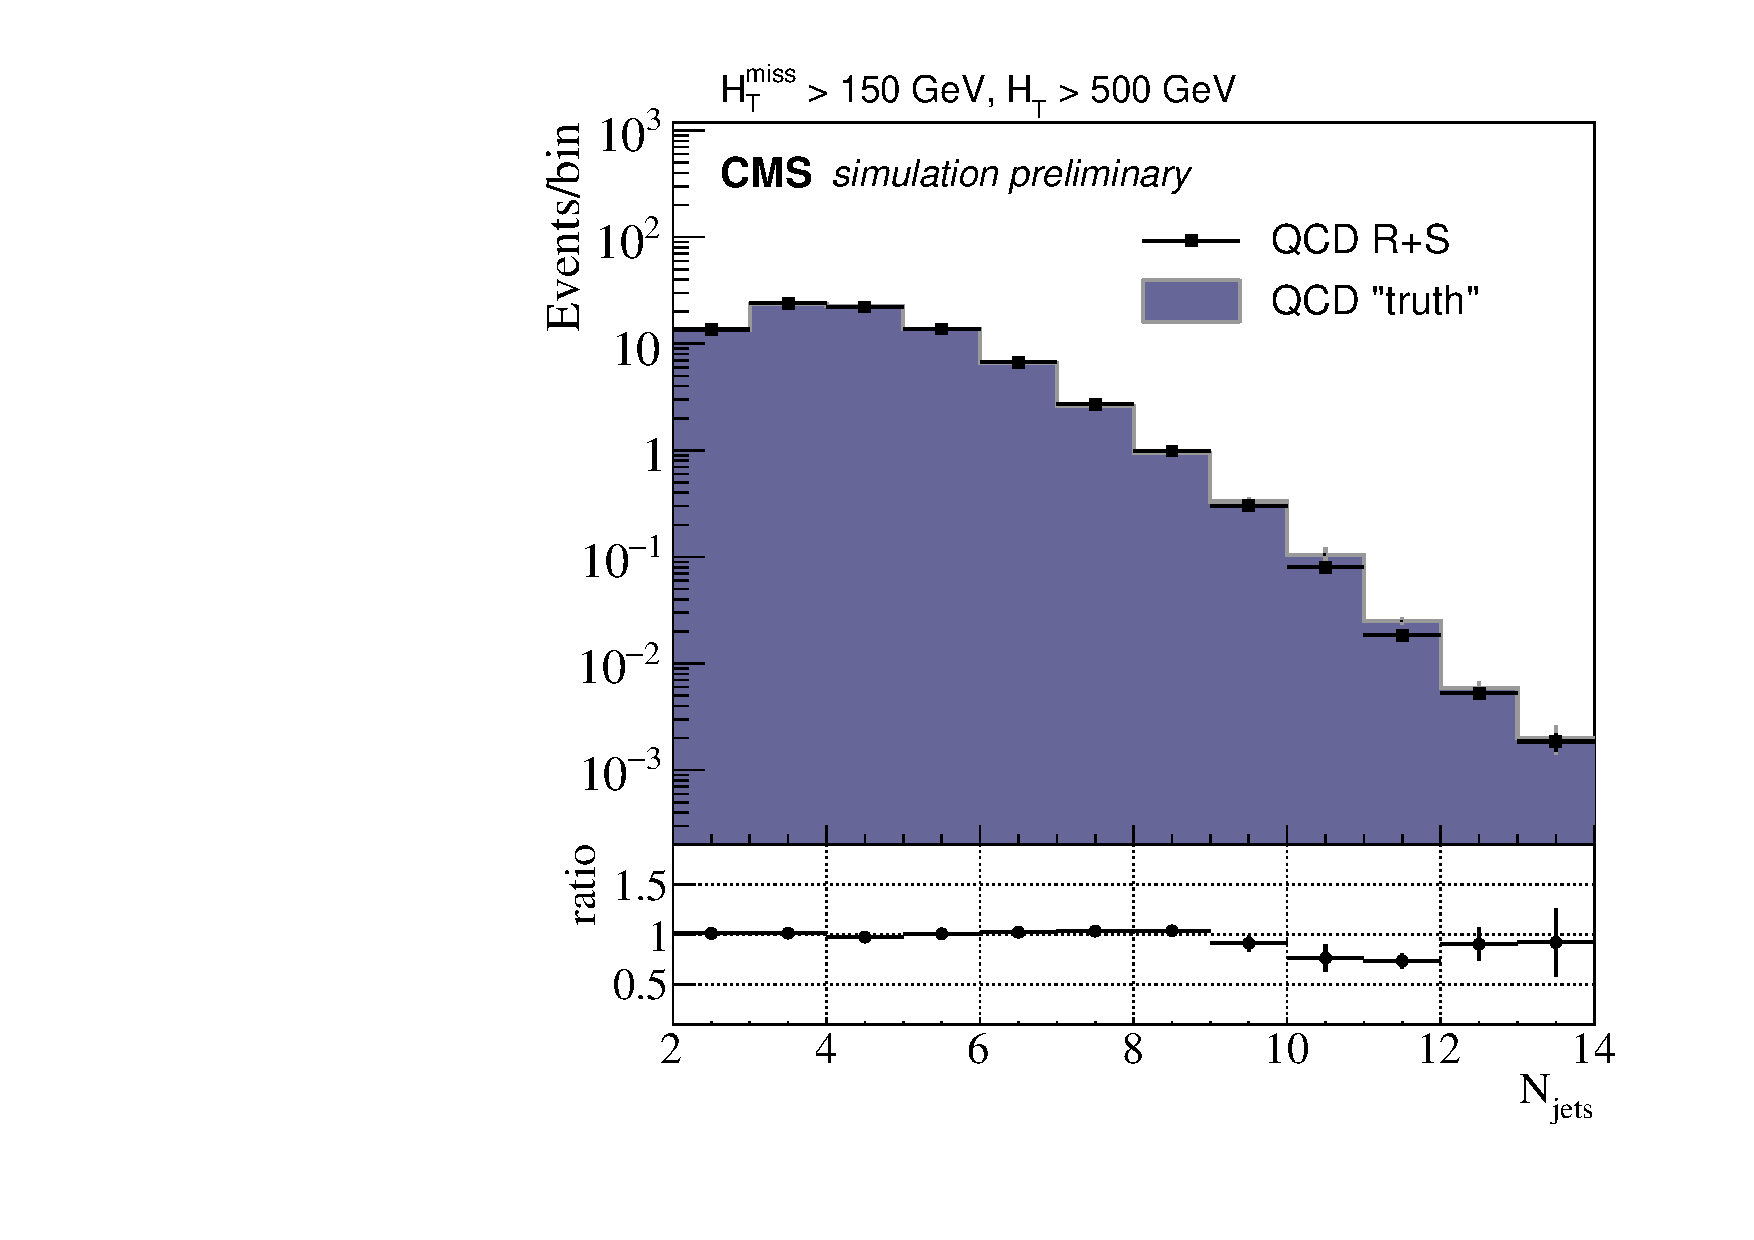
\includegraphics[width=0.5\linewidth]{figures/SusySearches/Ra2b2016/RplusSAndTruth_NJets.pdf}
}\\
\subfloat[]{
\includegraphics[width=0.5\linewidth]{figures/SusySearches/Ra2b2016/RplusSAndTruth_Mht.pdf}
}
\subfloat[]{
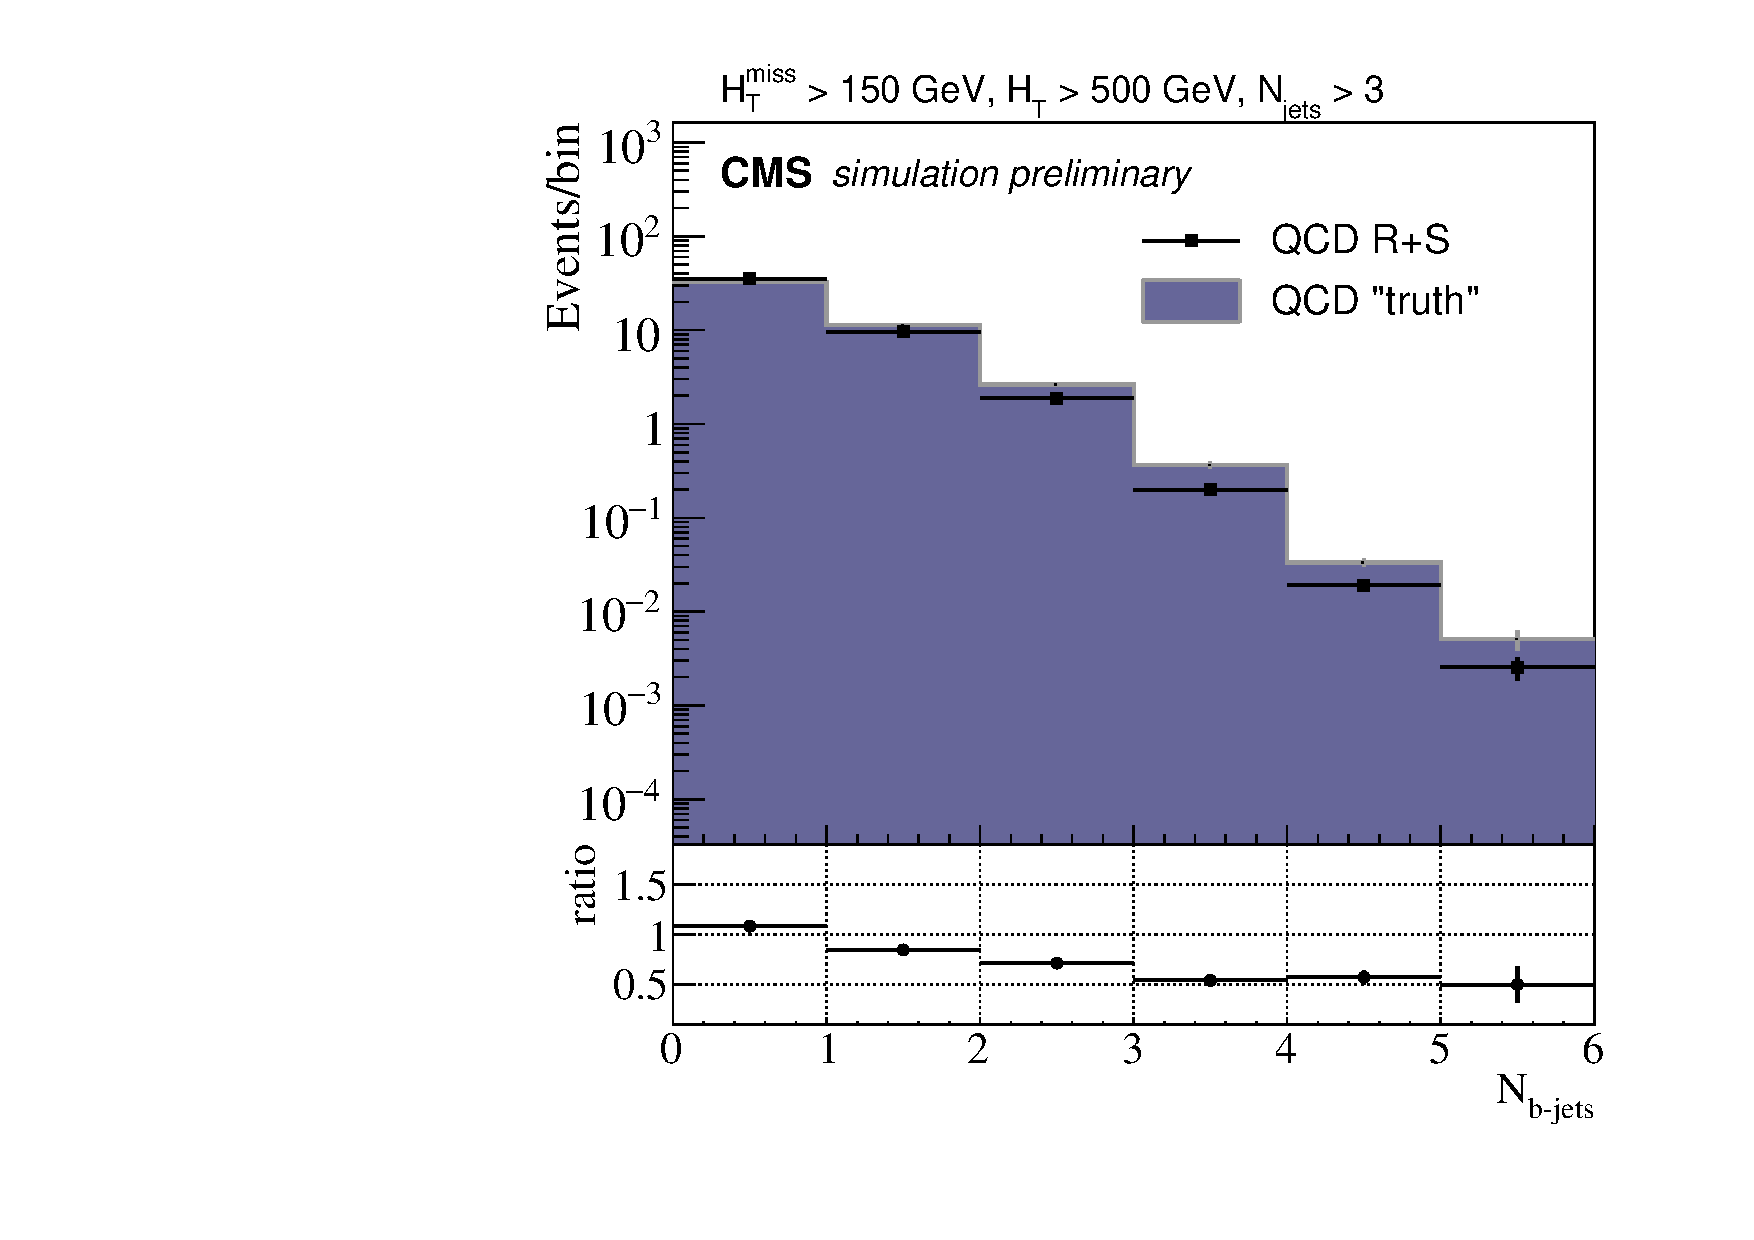
\includegraphics[width=0.5\linewidth]{figures/SusySearches/Ra2b2016/RplusSAndTruth_BTags.pdf}

}
\caption{Closure in simulation}
\label{fig:mg_muL}
\end{figure}

\begin{figure}[h]
\centering
\subfloat[]{
\includegraphics[width=0.5\linewidth]{figures/SusySearches/Ra2b2016/RplusSAndTruth_DPhiJet1Mht.pdf}
}
\subfloat[]{
\includegraphics[width=0.5\linewidth]{figures/SusySearches/Ra2b2016/RplusSAndTruth_DPhiJet2Mht.pdf}
}\\
\subfloat[]{
\includegraphics[width=0.5\linewidth]{figures/SusySearches/Ra2b2016/RplusSAndTruth_DPhiJet3Mht.pdf}
}
\subfloat[]{
\includegraphics[width=0.5\linewidth]{figures/SusySearches/Ra2b2016/RplusSAndTruth_DPhiJet4Mht.pdf}

}
\caption{Closure in simulation}
\label{fig:mg_muL}
\end{figure}

\begin{figure}[h]
\centering
\subfloat[]{
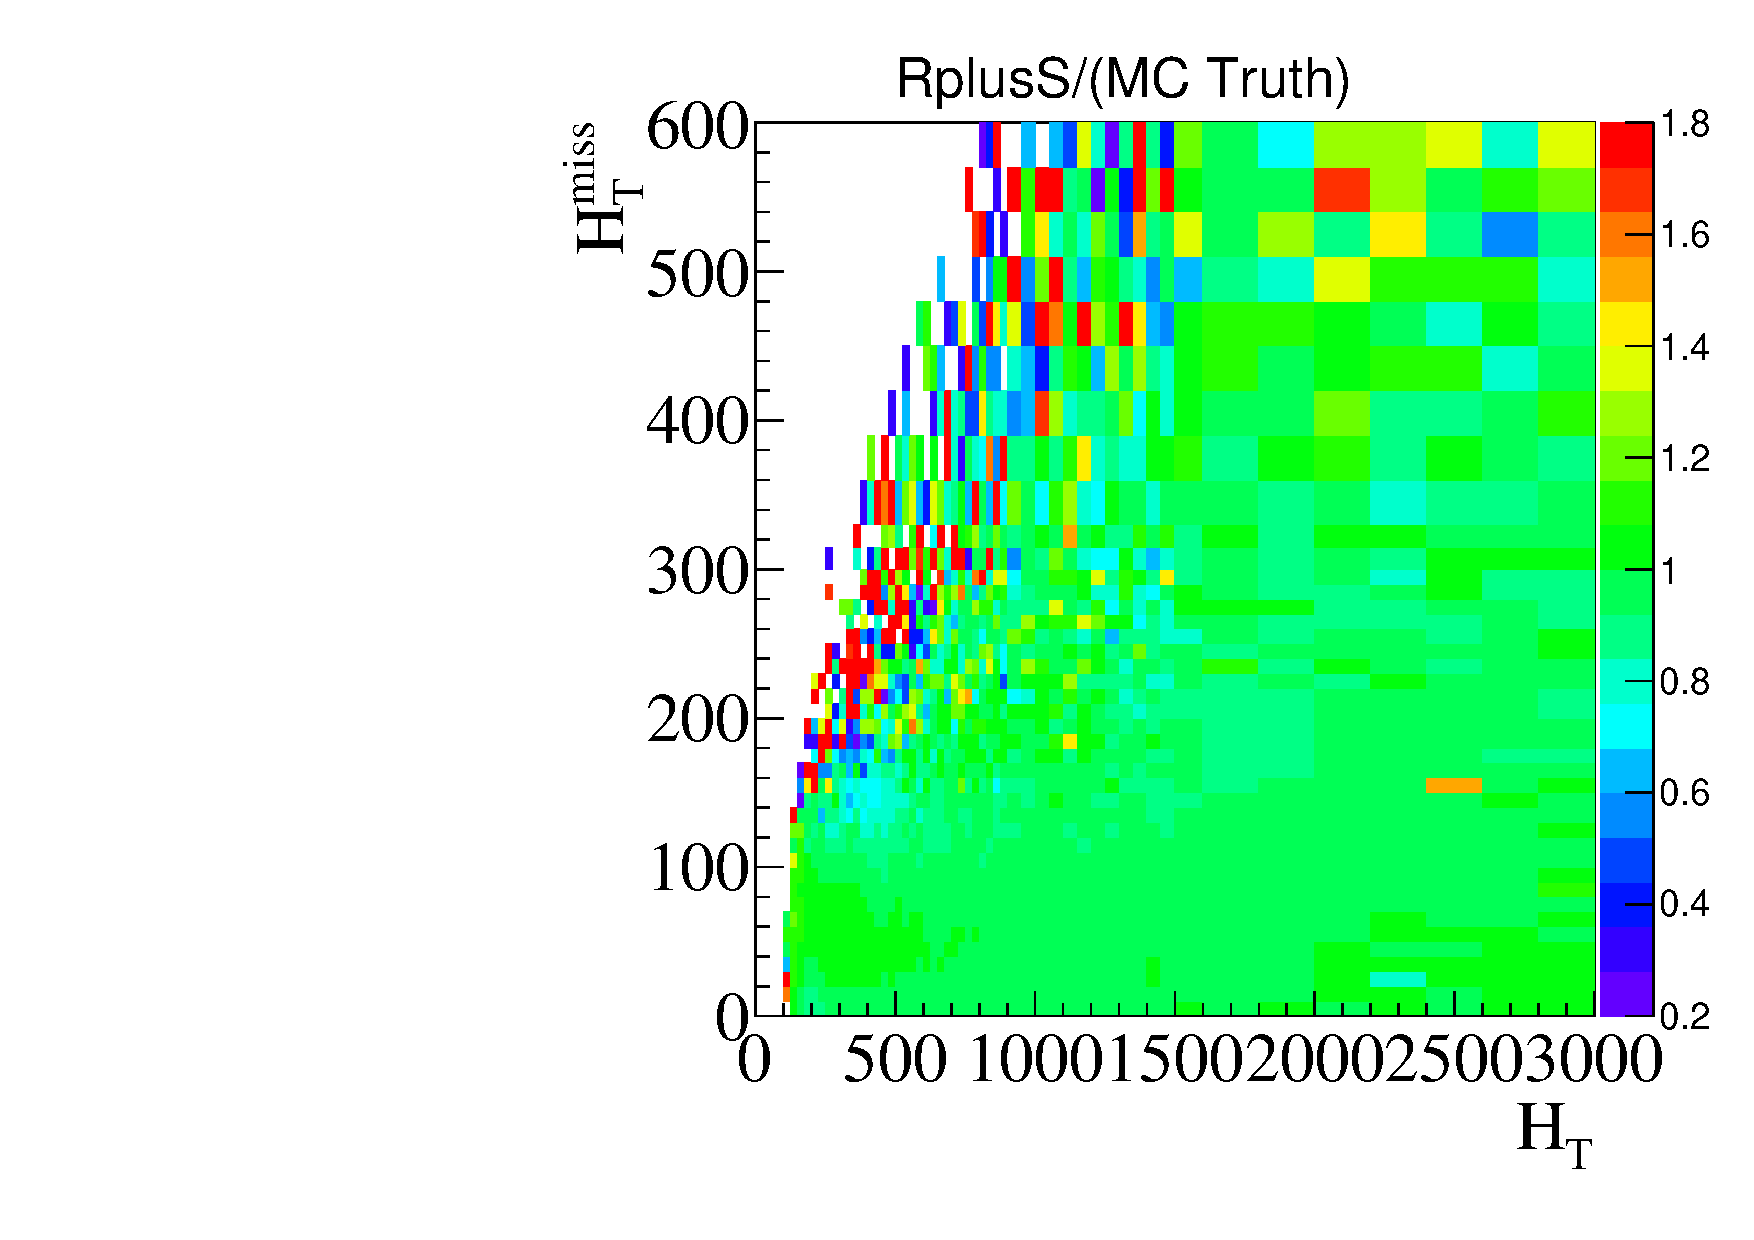
\includegraphics[width=0.5\linewidth]{figures/SusySearches/Ra2b2016/RplusSAndTruth_MhtVsHt.pdf}
}
\subfloat[]{
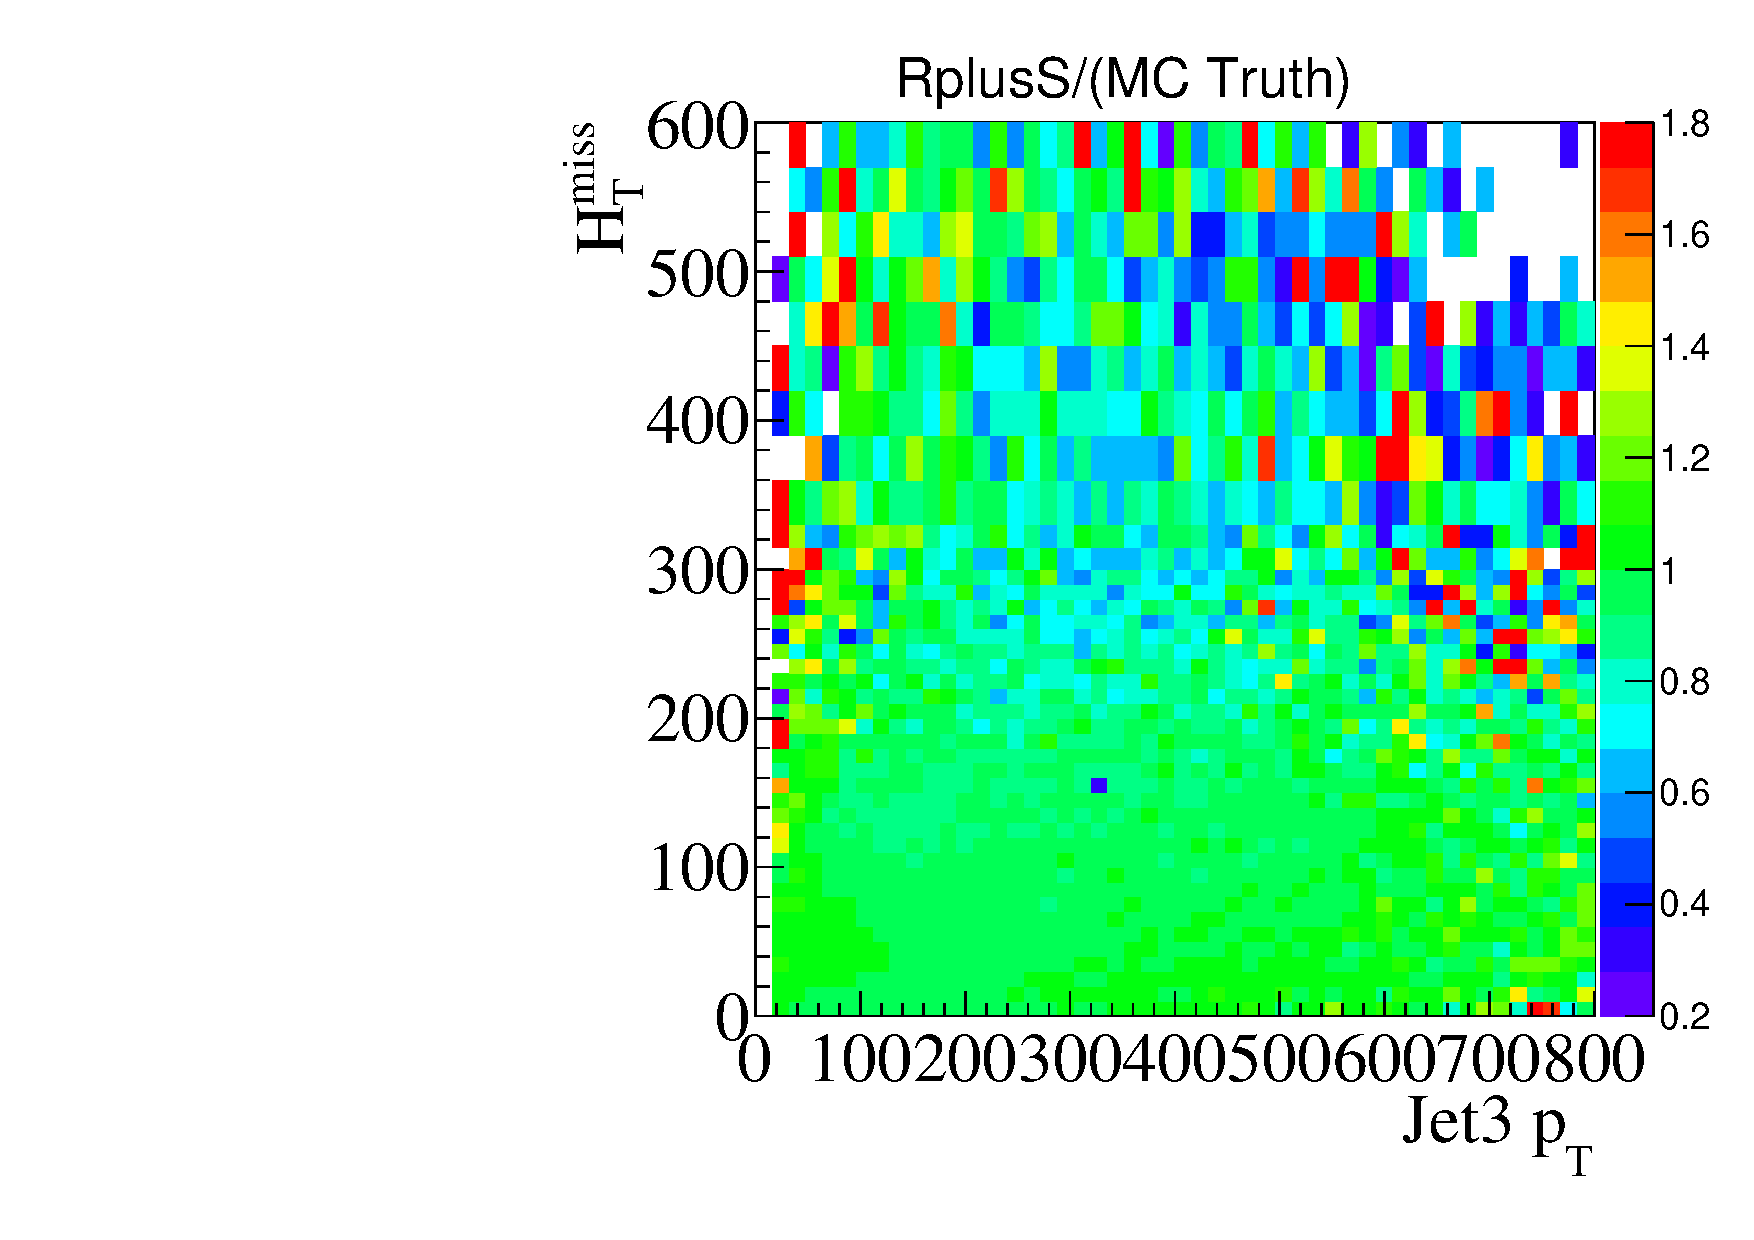
\includegraphics[width=0.5\linewidth]{figures/SusySearches/Ra2b2016/RplusSAndTruth_MhtVsJet3Pt.pdf}
}\\
\subfloat[]{
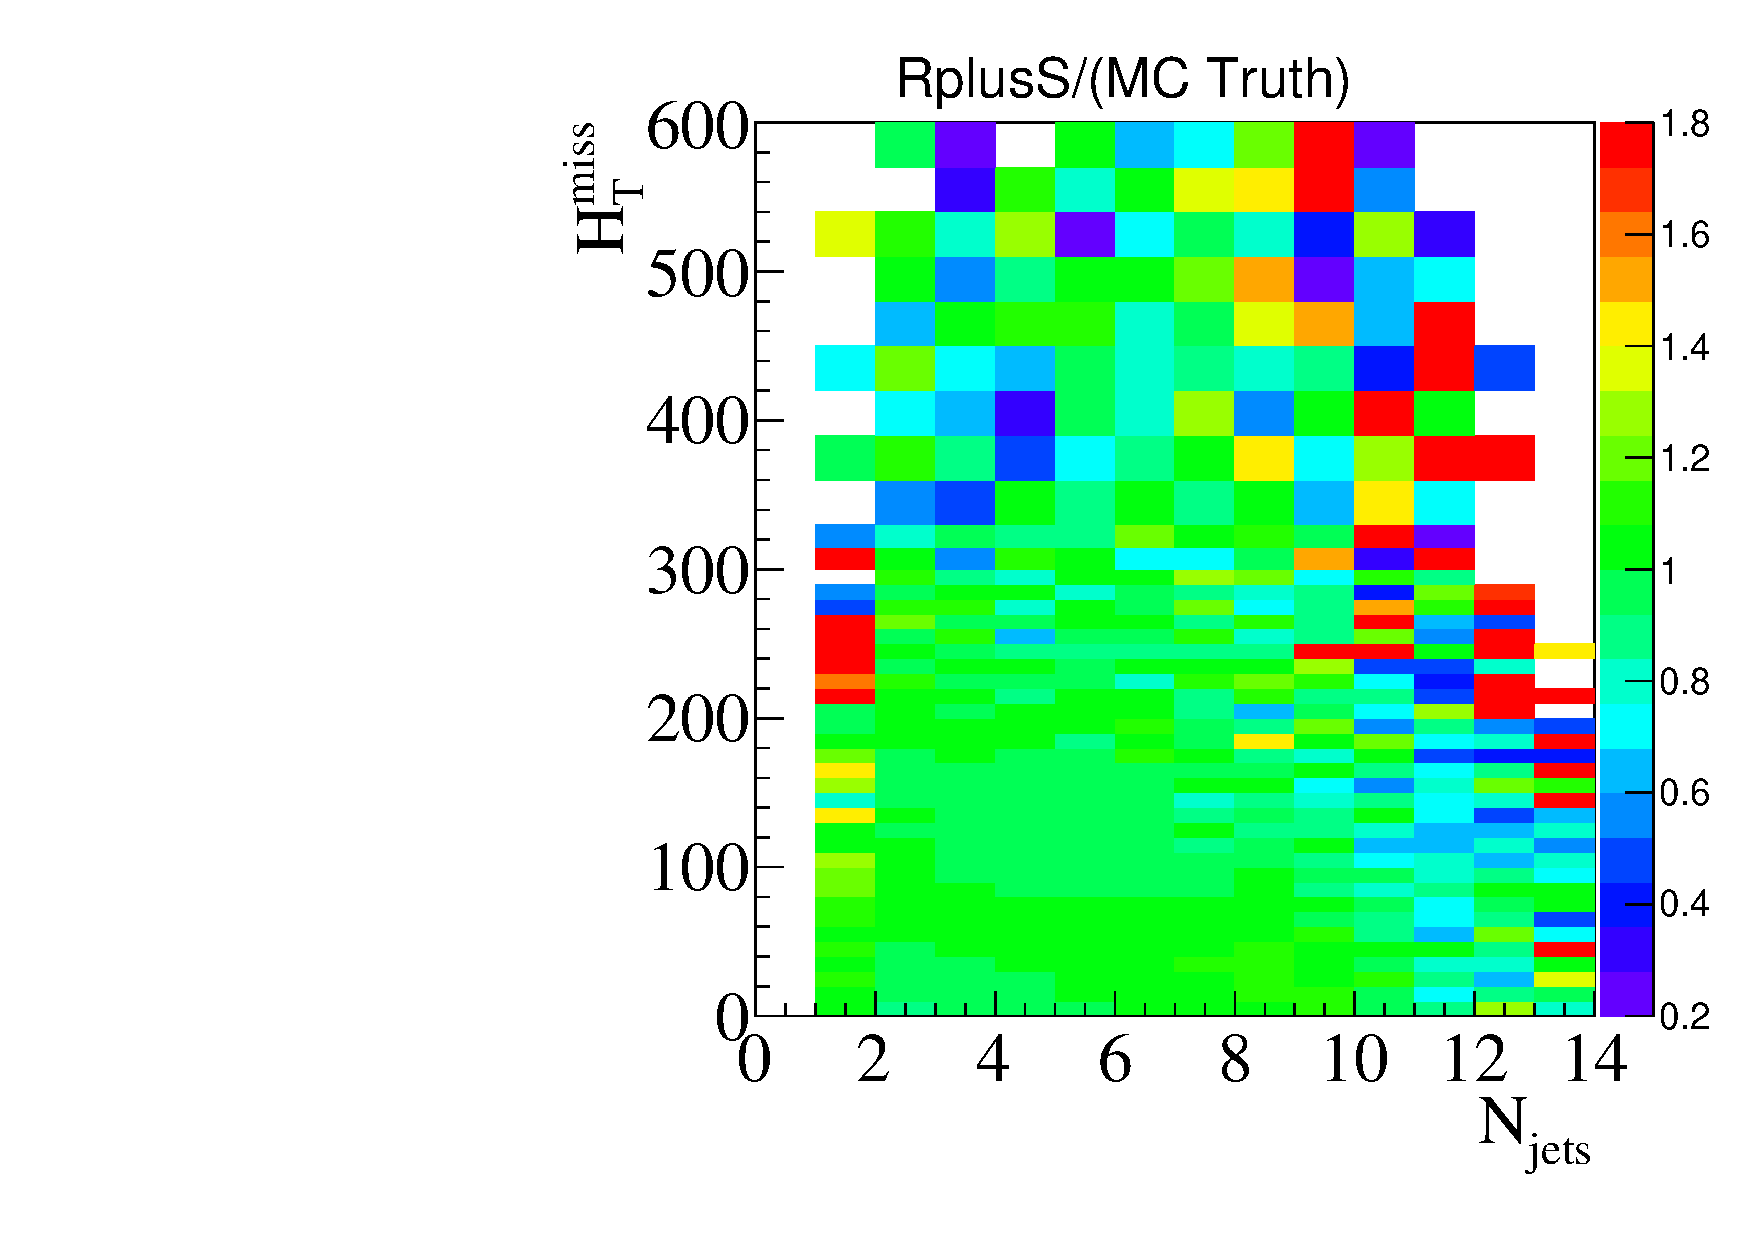
\includegraphics[width=0.5\linewidth]{figures/SusySearches/Ra2b2016/RplusSAndTruth_MhtVsNJets.pdf}
}
\subfloat[]{
\includegraphics[width=0.5\linewidth]{figures/SusySearches/Ra2b2016/RplusSAndTruth_MhtVsBTags.pdf}

}
\caption{Closure in simulation}
\label{fig:mg_muL}
\end{figure}

